%\documentclass[11pt,a4paper,runningheads]{llncs}
\documentclass[11pt,a4paper]{article}
%encoding
%--------------------------------------
\usepackage[T1]{fontenc}
\usepackage[utf8]{inputenc}
%--------------------------------------

%Portuguese-specific commands
%--------------------------------------
\usepackage[portuguese]{babel}
%--------------------------------------

%Hyphenation rules
%--------------------------------------
\usepackage{hyphenat}
\hyphenation{mate-mática recu-perar}
%--------------------------------------

\usepackage{graphicx}
\usepackage{comment}
\usepackage{pgfplots}
\usepackage{amsmath,amssymb,amsfonts}
\usepackage{algorithmic}
\usepackage{graphicx}
\usepackage{textcomp}
\usepackage{xcolor}
\usepackage{adjustbox}
\usepackage{float}
\usepackage{hyperref}


\begin{document}

\title{Fase 3 - Requisitos, Casos de Uso e Arquitetura}
\author{Pedro Carrega, nº49480 \and
Vasco Ferreira, nº49470 \and Ye Yang, nº 49521
}

%\institute{Departamento de Informática da Faculdade de Ciências da Universidade de Lisboa
%\email{\{fc49480,fc49470,fc49521\}@alunos.fc.ul.pt}}

\maketitle

\section{Motivação para Dataset e Serviços}

O dataset ecommerce foi escolhido pelo grupo devido ao grande número de eventos gerados e consequente informação produzida durante a utilização de uma loja de ecommerce. Informação esta que pode ser utilizada de diversas formas através de um grande número de variados serviços. Essa mesma informação poderá ser utilizada em vários contextos, sendo que escolhemos os seguintes 5 serviços que demonstram diferentes tipos de informação sobre o dataset:

\begin{itemize}
  \item api/products/listCategories: Fornece todas as diferentes categorias presentes nos dados
  \item api/products/popularBrands: Fornece a contagem de eventos associados a cada marca
  \item api/products/salesByBrand: Lista o numero de vendas de cada marca
  \item api/products/salePrice: Calcula o valor médio de venda de uma determinada marca
  \item api/events/ratio: Apresenta a distribuição relativa de cada tipo de evento, havendo os possíveis valores: view, cart e purchase
\end{itemize}

Os serviços foram escolhidos de forma a que consigam fazer diferentes tipos de operações sobre os dados, desde serviços mais específicos e por isso com menos carga na base de dados, a serviços mais abrangentes e consequente aumento de carga. Foram também escolhidos pois todos os serviços fornecem dados úteis para serem explorados no contexto de lojas de ecommerce.

\section{Diagrama de Casos de Uso}
\begin{figure}[H]
  \centering
    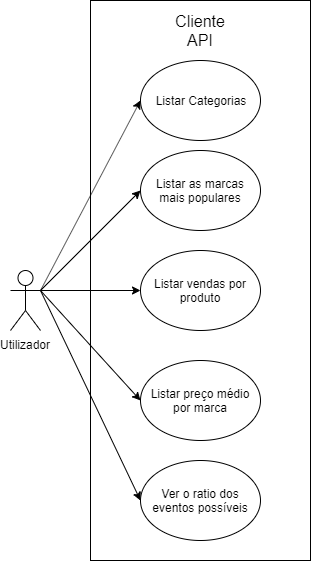
\includegraphics[scale=0.42]{Use_Cases.png}
  \caption{Diagrama de casos de uso}
\end{figure}

\section{Requisitos}

\begin{table}[H]
	\begin{center}
		\begin{tabular}{|p{3.5cm}|p{9.5cm}|}
		\hline
			\textbf{Requisitos\newline Não Funcionais} & \textbf{Descrição}\\ \hline
			Portabilidade & Implementação de servidor em NodeJS e cliente em HTML de modo a facilitar o processo de mudança de plataforma do serviço \\ \hline
			Legibilidade & A separação clara entre as camadas de apresentação, lógica de negócio e acesso à base de dados irá tornar o fluxo do sistema mais legível para os desenvolvedores \\ \hline
			Estabilidade & A distribuição do sistema por diversas máquinas virtuais, que poderão estar distribuídas por diferentes fornecedores cloud e em diferentes Data Centers permitem obter um sistema estável \\ \hline
			Elasticidade & O sistema deverá ser capaz de se adaptar à carga de trabalho através do provisionamento e desprovisionamento dos recursos de forma autónoma. Idealmente, de forma que em qualquer ponto do tempo, o sistema apenas utilize o número de máquinas necessárias de forma a corresponder à carga atual \\ \hline
			Escalabilidade & Capacidade do sistema lidar com o crescimento de carga de trabalho. Pode-se associar à capacidade de elasticidade do sistema \\ \hline
			Confiabilidade & Visto o sistema estar implementado na núvem, conseguimos garantir alta confiabilidade nos sistema, pois se um servidor no datacenter falhar, conseguimos facilmente migrar a VM para outro servidor funcional \\ \hline
	\end{tabular}
	\label{tab1}
	\end{center}
	\caption{Requisitos Não Funcionais}
\end{table}

\begin{table}[H]
	\begin{center}
		\begin{tabular}{|p{3.8cm}|p{8.2cm}|}
		\hline
			\textbf{Requisitos\newline Funcionais} & \textbf{Descrição}\\ \hline
			Listar\newline Categorias Disponíveis & Serviço que fornece aos clientes todas as categorias \\ \hline
			Visualizar\newline Popularidade das\newline Marcas & Serviço que fornece cada marca associada com a sua popularidade\\ \hline
			Visualizar\newline Número de Vendas\newline Individuais & Fornece o numero total de vendas de cada marca\\ \hline
			Visualizar\newline Preço Médio de Venda & Fornece o preço médio dos produtos vendidos de uma determinada marca \\ \hline
			Visualizar\newline Rácio de Tipo\newline de Eventos & Fornece a percentagem de cada tipo de evento \\ \hline
	\end{tabular}
	\label{tab2}
	\end{center}
	\caption{Requisitos Funcionais}
\end{table}

\section{Arquitetura da aplicação}
\begin{figure}[H]
  \centering
  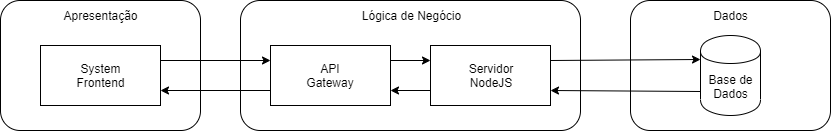
\includegraphics[scale=0.4]{App_arc.png}
  \caption{Arquitetura da aplicação}
\end{figure}

Após a definição da API na fase anterior, foi implementado de raiz um servidor em NodeJS que segue a API definida.


\subsection{Load Balancer}
Foi implementado um Load Balancer que distribui os pedidos HTTP recebidos dos clientes browser e que reencaminha para os respetivos serviços.


\subsection{Servidor NodeJS}
O servidor irá receber os pedidos a partir do Load Balancer, e processá-los de acordo com a funcionalidade pretendida. A lógica de negócio é aqui tratada, realizando as queries necessárias para a base de dados. Ao receber os dados, processa-os de acordo com a funcionalidade, e encaminha o resultado para o Load Balancer.
%\newline %removam isto se nao gostarem do espaço k adiciona

\subsection{Base de dados}
A base de dados irá conter o conteúdo dos ficheiros .csv do nosso dataset, que são acedidos pelo servidor de modo a poder efetuar as leituras necessárias para produzir uma resposta para o cliente. 
%\newpage

\section{Arquitetura técnica}
%Digam-me o que acham

%Não sei o que dizer da Portabilidade
Para garantir os requisitos não funcionais mencionados a cima devemos ter em atenção os serviços da cloud escolhidos, pois proporcionam vários aspetos fundamentais dos requisitos.
\newline

A utilização dos serviços disponibilizados pela AWS permite cumprir alguns dos requisitos não funcionais mencionados, nomeadamente a Escalabilidade e a Elasticidade. Já o Load Balancer implementado com o Ingress permite que este serviço da cloud trate automaticamente da separação dos diferentes tipos de pedidos HTTP recebidos para os respetivos serviços. A base de dados utilizada consiste uma imagem docker baseada na imagem mongo que como o nome sugere é uma imagem de MongoDB. Foi escolhida esta alternativa de forma a não estar dependente dos serviços de Bases de Dados de um fornecedor específico, sendo que com esta opção a imagem pode ser implementada numa instância em qualquer fornecedor cloud. Quanto à escalabilidade a imagem poderia ser replicada por diversas réplicas de forma a distribuir os pedidos feitos pelas diferentes réplicas.  %NOT TOTALY SURE,devemos por isto?
\newline

A Confiabilidade do sistema também é melhorada com a instalação em serviços na cloud, visto estas terem deteções automáticas de falhas de servidores, possibilitando a migração do sistema virtualizado para outro servidor funcional.
\newline

A Estabilidade é garantida nas várias ferramentas usadas na instalação do sistema. O Load Balancer como referido anteriormente faz a distribuição dos pedidos HTTP para os respetivos serviços, sendo que o Kubernetes atribui um DNS igual para todas as réplicas do serviço de maneira a que o Load Balancer apenas reencaminhe para o respetivo DNS, sendo o Kubernetes a distribuir a carga pelas respetivas réplicas do serviço. Isto permite que o sistema escale com facilidade já que aumentar o número de réplicas de um micro-serviço em Kubernetes é um processo rápido e sem necessitar de qualquer alteração no Load Balancer.
\newline

Já a Estabilidade é garantida devido a ter a Lógica de negócio distribuída por várias máquinas virtuais que cumprem a função de servidores.
\newline


A utilização do Docker permite-nos facilmente fazer deploy de um serviço, em qualquer máquina e em qualquer um fornecedor de cloud. Isto deve-se ao Dockerfile garantir a instalação de todas as dependências do serviço, variando conforme a linguagem de implementação do mesmo, cumprindo assim o requisito de Portabilidade do sistema.

\section{Implementação}

\section{Lançamento em Kubernetes}
O scripts de deployment do sistema foram separados em 4 devido à necessidade dos clusters e node groups estarem ativos, antes de proceder aos próximos passos. Existe também uma secção de edição de ficheiro manual, o que fez a quebra entre o terceiro e o quarto script.

Antes da execução dos scripts é necessário verificar a existência dos seguintes repositórios, roles e policies e caso existam, precisam de ser \textbf{eliminados}:
\begin{enumerate}
	\item Repositórios com nomes \textit{products} e \textit{events}
	\item AWS Role com nome eksServiceRole
	\item AWS Policy com nome ALBIngressControllerIAMPolicyEcommerce
\end{enumerate}

Para a execução dos scripts são necessárias as seguintes ferramentas:
\begin{itemize}
	\item AWS CLI
	\item eksctl
	\item kubectl
\end{itemize}

A região a escolher para o lançamento poderá ser qualquer um, porém recomendamos a região eu-west-1. Esta região terá de ser a mesma nos argumentos de todos os scripts que requeiram a mesma.

Com a utilização do Ingress, reparamos que existe a possibilidade deste poder usar VPCs antigas, para prevenir que tal ocorra, sugerimos apagar Target Groups que não estejam a ser utilizados.

\subsection{deploy1.sh}
O primeiro script de deployment recebe 3 argumentos na seguinte ordem:
\begin{enumerate}
	\item A região onde a Stack e o Cluster vão ser lançados (ex.: \textbf{eu-west-1})
	\item O nome da Stack que terá de ser único (nenhuma outra Stack na CloudFormation da conta pessoal poderá ter o mesmo nome) para o script funcionar corretamente (ex.:\textbf{ecommerce-stack})
	\item O nome do Cluster que também terá de ser único (ex.:\textbf{ecommerce-cluster})
\end{enumerate}

A criação da stack e do cluster irá demorar cerca de 10 a 20 minutos até ficarem ativos, após o qual poderemos proceder à execução do segundo script. O estado do script pode ser verificado com o seguinte comando:
\begin{itemize}
	\item \textit{aws eks describe-cluster \texttt{-{}-}name CLUSTER\_NAME} , mudando CLUSTER\_NAME para o nome do cluster dado nos argumentos
\end{itemize}
A execução do segundo script só deve ser feita quando o estado do cluster estiver em \textbf{ACTIVE}.

\subsection{deploy2.sh}
O segundo script recebe os mesmos argumentos que o primeiro, todos na mesma ordem. Neste script vão ser criados os node groups e o pull das imagens dos serviços.

Para realizar o pull, irá ser pedido para inserir os credenciais IAM que dão acesso aos repositórios por nós criados. Estes credenciais encontram-se no ficheiro \textbf{credenciais.txt} juntamente com a região onde os repositórios se encontram.

No fim da execução do script, é necessário verificar o estado dos node groups antes de proceder ao próximo script. O estado pode ser verificado com o seguinte comando: 
\begin{itemize}
	\item \textit{aws eks describe-nodegroup \texttt{-{}-}cluster-name CLUSTER\_NAME \texttt{-{}-}nodegroup STACK\_NAME} , mudando CLUSTER\_NAME e STACK\_NAME para os respetivos nomes dados nos argumentos
\end{itemize}
No final irá ser pedido para introduzir os credenciais de IAM para a conta de AWS pessoal de modo a poder criar os repositórios e fazer push das imagens no script seguinte.
Após o estado do node group passar para \textbf{ACTIVE} podemos proceder À execução do terceiro script.

\subsection{deploy3.sh}
O terceiro script recebe 2 argumentos na seguinte ordem:
\begin{itemize}
	\item A região que deverá ser idêntica às inseridas nos scripts anteriores
	\item O nome do cluster que também deverá ser o mesmo
\end{itemize}
Para a correto funcionamento deste script, salienta-se a necessidade de apagar os repositórios, roles e policies anteriormente referidos.

Após a criação dos repositórios e o push das imagens para os mesmos, será pedido para mudar os credenciais IAM para os que se encontram no ficheiro \textbf{credenciais\_mongo.txt} para realizar o pull da imagem da base de dados.

Depois de realizar o pull irá ser pedido para mudar os credenciais de novo para a conta pessoal de AWS para a criação do repositório da base de dados e o push da imagem.

\subsection{deploy4.sh}
Antes da execução do 4 ficheiro de deployment, as seguintes mudanças terão de ser realizadas nos ficheiros \textbf{ingress/ingress-rbac.yaml} e \textbf{ingress/alb-ingress-controller.yaml}.

\subsubsection{ingress/ingress-rbac.yaml}
Neste ficheiro é necessário inserir manualmente os dados relativos ao role criado no ficheiro na seguinte linha:
\begin{itemize}
	\item \textbf{eks.amazonaws.com/role-arn:}
\end{itemize}
Para aceder ao valor do ARN do role criado, basta inserir na linha de comandos as seguintes instruções:
\begin{itemize}
	\item \textbf{aws iam get-role \texttt{-{}-}role-name eksServiceRole}
\end{itemize}

\subsubsection{ingress/alb-ingress-controller.yaml}
Neste ficheiro é necessário inserir a informação relativa ao cluster criado para que o Ingress utilize os recursos corretos. Para tal é necessário alterar no ficheiro, na linha \textbf{- \texttt{-{}-}cluster-name=CLUSTER\_NAME},
alterando \textbf{CLUSTER\_NAME} pelo nome do cluster dado nos argumentos dos scripts anteriores.

Após a execução destes 2 passos, executa-se o quarto e último script, \textbf{deploy4.sh} sem parâmetros de entrada.

\subsection{Acesso aos serviços}
Após a aplicação dos ficheiros yaml do Ingress, é possível aceder ao sistema executando o comando:
\begin{itemize}
	\item \textbf{kubectl get ingress}
\end{itemize}
Deste comando retira-se o endereço que se encontra em \textit{Address} e adiciona-se os paths para os serviços disponibilizados (ex.: <address>/api/products/listCategories).

\subsection{Desconstrução do deployment}
Para remover a montagem do sistema, seguem-se os seguintes passos:
\begin{enumerate}
	\item Na consola de EKS \url{https://eu-west-1.console.aws.amazon.com/eks/home?region=eu-west-1#/clusters}, dependendo da região escolhida, selecionar o cluster e apagar o node group correspondente. Após dos node groups terem sido eliminados, proceder com a eliminação do cluster.
	\item Na consola de EC2 \url{https://eu-west-1.console.aws.amazon.com/ec2/v2/home?region=eu-west-1#LoadBalancers}, eliminar os load balancers criados. Na mesma consola navegar para os target groups e apagar aqueles que estejam relacionados com o VPC criado.
	\item Na consola de VPC \url{https://eu-west-1.console.aws.amazon.com/vpc/home?region=eu-west-1#NatGateways}, eliminar as NATs criadas. Após a eliminação, navegar para a secção dos VPCs e eliminar as VPCs correspondentes que contém o nome dado à stack.
	\item Na consola de ECR \url{https://console.aws.amazon.com/ecr/repositories?region=us-east-1}, eliminar os seguintes repositórios: \textit{database}, \textit{events} e \textit{products}.
	\item Na consola de IAM Policies \url{https://console.aws.amazon.com/iam/home?#/policies}, eliminar a policy com o seguinte nome: \textbf{ALBIngressControllerIAMPolicyEcommerce}. Após a eliminação, navegar para a secção dos Roles, e apagar o role com o seguinte nome: \textbf{eksServiceRole}.
	\item Na consola de CloudFormation \url{https://eu-west-1.console.aws.amazon.com/cloudformation/home?region=eu-west-1#/stacks}, eliminar a stack criada com o nome dado nos scripts anteriores.
\end{enumerate}

\end{document}